\subsection{OR-ing Module (OR) }
\label{sec:OR}

The OR-ing Module (OR) combines the outputs of SI\textsubscript{1} and  SI\textsubscript{2}.


\subsubsection{Requirements}

The contribution of both panels should be summed.

\subsubsection{Implementation}

S\textsubscript{1'} and .S\textsubscript{2'} are connected.



\begin{figure}[h]
    \centering
    
\includegraphics[width=0.3\textwidth]{PO/OR/OR}
    %\caption{SI - schematic, n = 1,2}
\end{figure}


\begin{table}[H]
    \centering
    \begin{threeparttable}[b]
        \begin{tabularx}{\linewidth}{ >{\hsize=.15\hsize}X >{\hsize=1.35\hsize}X >{\hsize=1.5\hsize}X }
            \toprule
            Id & Issue                                       & Potential solutions    \\
            \midrule
            1  & only one panels contributes at a given time & separate charger units \\
            \bottomrule
        \end{tabularx}
    \end{threeparttable}
    \caption{OR - issues}
\end{table}



\subsubsection{LiPo Charger}

Net \cb{net}{.S\textsubscript{'\lor}} is connected to \texttt{SOLAR IN +} of the charger shown in Fig.\ref{fig:wv}.

\begin{figure}[h]
    \centering
    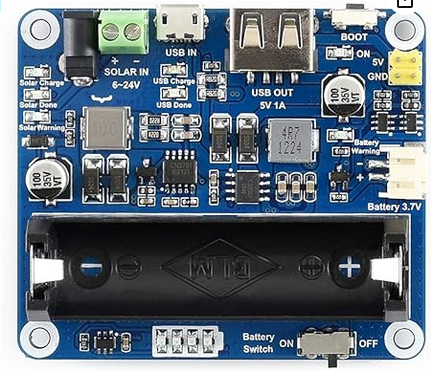
\includegraphics[scale=0.4]{charger}
    \caption{Waveshare solar power LiPo charger}
    \label{fig:wv}
\end{figure}